\documentclass[letterpaper,12pt,addpoints]{exam}


% \usepackage{fancyhdr}
\usepackage[utf8]{inputenc}
\usepackage{microtype}
\usepackage[top=1in, bottom=1in, left=1in, right=1in]{geometry}
\usepackage{graphicx}
\usepackage{siunitx}
\newcommand{\celsius}{\si{\celsius }}
\newcommand{\kelvin}{\si{\kelvin}}
\newcommand{\sub}[1]{\textsubscript{#1}}
\newcommand{\super}[1]{\textsuperscript{#1}}

\usepackage{hyperref}
\usepackage{amsmath}
\usepackage{enumitem}

\renewcommand{\bigskip}{\vspace{1in}}
\newcommand{\hugeskip}{\vspace{2in}}
\newcommand{\giantskip}{\vspace{3in}}
\sisetup{retain-explicit-plus}

\newcommand{\university}{Samford University}
\newcommand{\faculty}{Department of Physics}


\newcommand{\content}{Example Content}

\newcommand{\timelimit}{65 minutes}
\newcommand{\myline}{\vspace{.5cm}\hrule}
\newcommand{\week}{}

%\pagestyle{fancy}
%\setlength\parindent{0in}
%\setlength\parskip{0.1in} 
%\setlength\headheight{15pt}





%\pagestyle{headandfoot}
%\firstpageheader{}{}{}
%\firstpagefooter{}{Page \thepage\ of \numpages}{}
%\runningheader{\class}{\examnum}{\examdate}
%\runningheadrule
%\runningfooter{}{\thepage}{}

\title{\vspace{-3cm}\class}
\author{\examnum}
\date{\examdate}


%%%%%%%%%%% HEADER / FOOTER %%%%%%%%%%%
\rhead{\examnum}
\chead{\textsc{}}
\lhead{\textsc{\class}}
\rfoot{\textsc{\thepage}}
\cfoot{\textit{}}
\lfoot{\textsc{\university}}
%%%%%%%%%%%%%%%%%%%%%%%%%%%%%%%%%%%%%%%

\pagestyle{headandfoot}
\firstpageheader{\textsc{\class}}{}{\examnum}
\firstpageheadrule
\firstpagefooter{\textsc{Samford University}}{\examdate}{\textsc{Total Points}: \numpoints}
\runningheader{\textsc{\class}}{}{\textsc{\examnum}}
\runningheadrule
\runningfooter{}{}{\thepage}

\setlength{\parindent}{0pt}
\setlength{\parskip}{\baselineskip}

\title{\class}
\author{\examnum}
\date{\examdate}

\newcommand{\class}{Phys420 - Thermal Physics}
\newcommand{\examnum}{Exam 1}
\newcommand{\examdate}{Due 2024/10/01 at 9:00am}

\begin{document}
	\addpoints
	
	\textsc{Instructions:} You must work with your own effort in the following problems. You may not seek the help of any other humans or computers, either in the past or present with the following exceptions: mathematical facts using either standard references or tables and texts or \emph{Mathematica}, your notes or my notes, and your textbook. You must cite the source of any mathematical facts outside of my notes or your textbook that you use. 
	
	Work the problems in the space provided but feel free to use more sheets. Also turn in any spread sheets or other files you use to do calculations. Most of all, be clear and neat in the work you turn in. You are presenting a case to me so it needs to be easy to follow your argument. 
	
	\begin{questions}
		\setlength\itemsep{1 in}
		
		\question
		In your own words, state or summarize the following:
		\begin{parts}
			\part[2] 0th Law of Thermodynamics
			\vspace{2cm}
			\part[2] 1st Law of Thermodynamics
			\vspace{2cm}
			% \part[2] 2nd Law of Thermodynamics
			% \vspace{2cm}
			\part[2] An adiabatic compression
			\vspace{2cm}
			\part[2] An isobaric expansion
			\vspace{2cm}
			\part[2] An isochoric process
			\vspace{2cm}
			\part[2] An isothermal compression
			\vspace{2cm}
			\part[2] What is an example of a process where heat is given to the system but the system's temperature remains the same?
		\end{parts}
		%\clearpage
		
		\question[5]
		At what temperature does the Fahrenheit scale and the Kelvin scale read the same number? Show your work.
		
		\vspace{3in}
		
		\question[5]
		During an isobaric expansion of an ideal gas, does the temperature of the gas increase or decrease? Provide a good explanation of this. 
		
		\newpage
		\question[5]
		Show that $\gamma = \dfrac{C_p}{C_v}$. 		
		
		\vspace{3in}
		\question[5] You have two cubes of materials that have equal dimensions each with side length of \SI{3.93}{inches}. One is steel and one is porcelain. Very quick googling tells me that steel has a density of \SI{7.85}{\gram \per \centi\meter^3} and a specific heat of \SI{466}{J/kg K} while porcelain has a density of \SI{2400}{\kilo\gram \per \meter^3} and a specific heat of \SI{1.085}{\joule \per \gram \per \kelvin}. How much heat is needed to change the temperature of each of these samples by \SI{1}{\celsius}? (\emph{HINT: Dear Lord, be careful with units...})
		
		\newpage
		\question 
		Look around in our classroom (Propst 011) and think of the air as all N\sub{2}.
		\begin{parts} 
			\part[5] Circle one of the following that is the best estimate for the volume of our classroom and justify your answer.
			\begin{itemize}
				\item 3 \si{\meter^3}
				\item 30 \si{\meter^3}
				\item 300 \si{\meter^3}
				\item 3000 \si{\meter^3}
			\end{itemize}
			\part[5] Using your volume estimate, calculate the number of moles of air in the room and the total number of molecules. Assume it is atmospheric pressure and room temperature of 20\si{\celsius} and that it is all N\sub{2} molecules.
			\part[5] What is the root-mean-square velocity of the (N\sub{2}) molecules in the room?
			\part[5] What is the internal energy of the air in the room?
			\part[5] What is the average energy \emph{per particle} of the air in the room?
			%\part[5] What is the entropy of the air in the room?
		\end{parts}
		\clearpage
		
		\question
		\begin{parts}
			\part[10] A monatomic gas at room temperature and atmospheric pressure is adiabatically compressed to 1/20th its original volume. What is the final temperature \emph{in Fahrenheit} and are you surprised by this? Comment on your surprise.
			\part[10] What is the final pressure of this gas?
			\part[10] How much work was done on this gas?
			%\part[10] Calculate the change in entropy for this process (assuming it is a reversible, quasistatic compression) and comment on your surprise at it too. 
			
		\end{parts}
		
		\clearpage
		
		\question
		For the PV diagram below, an isothermal process connects points A and B, followed by an isobaric to point C and an isochoric process back to point A. Answer the following questions in terms of $P_1, P_2, V_1, V_2$: \newline
		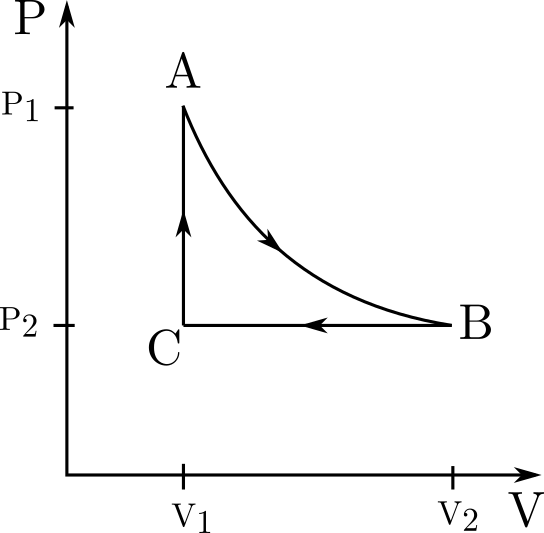
\includegraphics{PV-1.png}
		\begin{parts}
			\part[4] How much work is done between point A and B.
			\part[4] How much work is done between point B and C.
			\part[4] How much work is done between point C and A.
			\part[4] How much heat is added or removed from point A to point B.
			\part[4] How much heat is added or removed from point C to point A.
			\part[4] What is the total change in internal energy of the complete cycle?
			\part[4] Is the work done on the gas positive or negative?
		\end{parts}
		\clearpage
		
		%\question
		%\begin{parts}
		%\part[10] Derive an expression for the multiplicity of an Einstein solid in the low temperature limit ($q<<N$) starting with the formula $$\Omega(N,q) = \frac{(q+N-1)!}{q!(N-1)!}$$ and applying Stirling's approximation in the form $$\ln N!\approx N \ln N - N.$$
		%\part[10] Find the entropy for an Einstein solid with $q=10^{20}$ and $N=10^{23}$ and compare this to the entropy of a Einstein solid in the high temperature limit for $q=10^{25}$ and $N=10^{23}$. 
		%\end{parts}
		
		\clearpage
		
		\question[10] If 500 grams of 0\si{\celsius} ice in a styrofoam cup is filled up with 200 grams of 20\si{\celsius} sweet tea, then how much of the ice melts? (Specific heat capacity of water is 4.2 \si[per-mode=symbol]{\joule\per\gram\per\kelvin} and the latent heat for melting ice is 333 \si{\joule/\gram}.)
		
	\end{questions}
\end{document}
